
%(BEGIN_QUESTION)
% Copyright 2008, Tony R. Kuphaldt, released under the Creative Commons Attribution License (v 1.0)
% This means you may do almost anything with this work of mine, so long as you give me proper credit

Etter at innsiden av dette forbrenningskammeret er foret med helt nye ildfaste steiner, må det varmes opp sakte til full temperatur. Denne langsomme oppvarmingsprosessen kalles {\it curing}. Hvis oppvarmingen går for raskt, kan damptrykket fra intern fuktighet i steinene få dem til å sprekke eller til og med eksplodere. Den viktigste grensen å passe på i starten av curing av nytt ildfast foringsmateriale er ikke maksimal temperatur, men maksimal temperatur-{\it rate}.

$$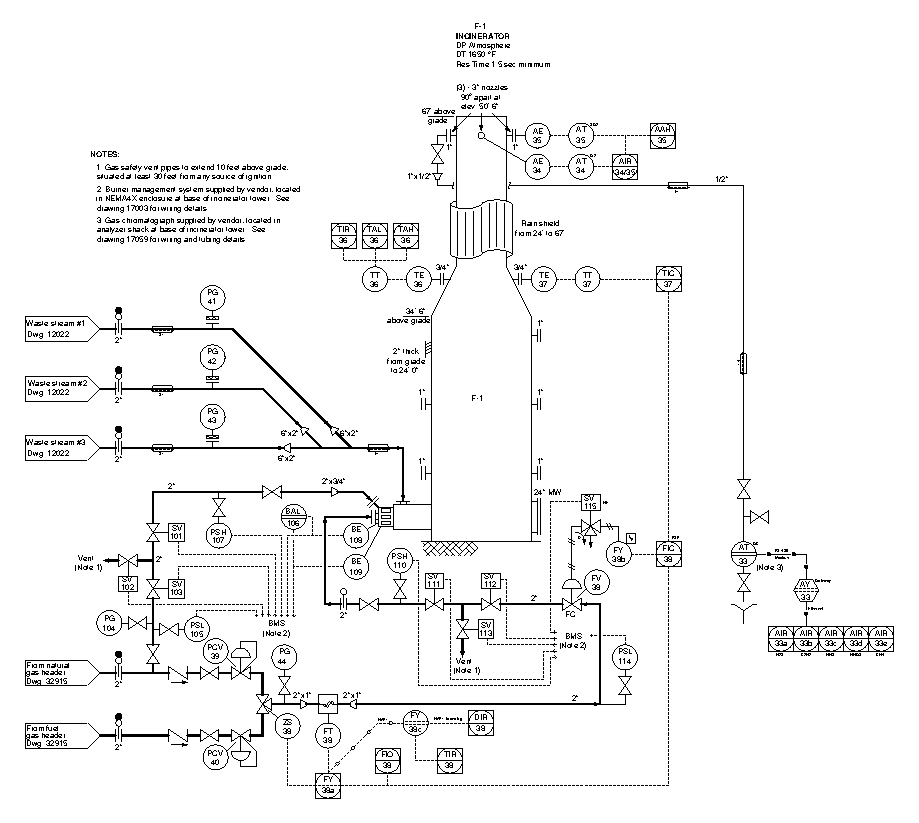
\includegraphics[width=15.5cm]{i0004rx01.eps}$$

Hvis du observerer grafen fra trendregistrator TIR-36, hvilke trekk i grafen vil vise deg {\it raten} for temperaturøkning? Vær så konkret som mulig i svaret, gjerne med et tall-eksempel. Bestem også måleenheten for en temperatur-endringsrate.

Oppgi også ISA-tagbokstaven som brukes for instrument som måler eller virker på {\it endringsraten} til en variabel, og hvor du ville installert et slikt instrument i dette systemet for å hjelpe driftspersonell med å overvåke temperaturøkningstakten i forbrenningskammeret.

\vskip 20pt \vbox{\hrule \hbox{\strut \vrule{} {\bf Forslag til sokratisk diskusjon} \vrule} \hrule}

\begin{itemize}
\item{} Beskriv hvordan man ville programmert et styresystem, for eksempel et DCS, til å beregne {\it rate} av temperaturendring for å varsle personell nær ovnen dersom denne raten blir for høy. Hvilke matematiske trinn må styresystemet utføre for å beregne en endringsrate fra påfølgende temperaturmålinger?
\end{itemize}

\underbar{file i01507}
%(END_QUESTION)





%(BEGIN_ANSWER)


%(END_ANSWER)





%(BEGIN_NOTES)

Å beregne endringsrate over tid er like enkelt som å beregne helning: {\it stigning} over {\it løp}. I dette tilfellet:

$$\hbox{Helning} = {dT \over dt}$$

Hvis disse helningene beregnes manuelt mellom diskrete tidspunkter i stedet for kontinuerlig av en analog datamaskin, er ligningen i praksis:

$$\hbox{Helning} = {\Delta T \over \Delta t}$$

Måleenheten for endringsrate er sammensatt: temperaturenhet per tidsenhet. For eksempel grader (F eller C) per minutt.

\vskip 10pt

ISA 5.1-standarden reserverer bokstaven ``K'' for endringsrater. Dermed kan dette forbrenningskammeret utstyres med en indikator for temperatur-endringsrate kalt TKI-36. Alarmenheter som overvåker temperatur-endringsrate kan merkes TKAH-36 (og eventuelt TKAL-36 dersom vi også er opptatt av høy rate for temperatur{\it fall} i tillegg til høy rate for temperatur{\it økning}).










\vskip 20pt \vbox{\hrule \hbox{\strut \vrule{} {\bf Virtuell feilsøking} \vrule} \hrule}

Denne oppgaven egner seg godt som en ``Virtuell feilsøking''-øvelse. Når du presenterer diagrammet for studentene, ser du først for deg en bestemt feil i systemet. Deretter presenterer du ett eller flere symptomer på feilen (noe en operatør eller annen bruker kan observere). Studentene foreslår så ulike diagnostiske tester for å identifisere type og plassering av feilen, som om de var teknikere som feilsøker problemet. Din oppgave er å fortelle hva resultatet ville blitt av hver foreslåtte test, og dokumentere resultatene slik at alle studentene kan se dem.

Under og etter øvelsen er det nyttig å stille oppfølgingsspørsmål som:

\begin{itemize}
\item{} Hva forteller resultatet av den siste diagnostiske testen om feilen?
\item{} Anta at resultatene av den siste diagnostiske testen var annerledes. Hva ville det resultatet da fortelle om feilen?
\item{} Er den siste diagnostiske testen den beste vi kunne utført?
\item{} Hva ville vært den ideelle rekkefølgen av tester for å diagnostisere problemet med færrest mulige trinn?
\end{itemize}

%INDEX% Mathematics, calculus: rate of temperature rise
%INDEX% Process: incinerator (realistic P\&ID shown)

%(END_NOTES)
